\documentclass[12pt]{article}
\usepackage[utf8]{inputenc}
\usepackage{graphicx}  % For including figures
\usepackage{amsmath}   % For math symbols
\usepackage{amssymb}   % For math symbols
\usepackage{hyperref}  % For clickable links
\usepackage{geometry}  % For setting margins
\usepackage{setspace}  % For setting line spacing
\usepackage{fancyhdr}  % For customizing headers
\usepackage{cite}      % For bibliography
\usepackage{lipsum}    % For placeholder text
\usepackage{titlesec}  % For subsection formatting
\usepackage{booktabs}  % For table lines
\usepackage{tikz}      % For drawing graphs
\usepackage{caption}   % For captions
\usepackage{float}     % For placing figures
\usepackage{subcaption} % For subfigures

\newcommand{\subsubsubsection}[1]{
  \vspace{1em} % Space above the section
  \noindent\textbf{#1} % Bold the section title
  \vspace{0.5em} % Space below the section
}

\geometry{letterpaper, margin=1in}
\setstretch{1.5}  % 1.5 line spacing

\begin{document}

\tableofcontents

\newpage

\section{Notation}

\begin{table}[ht]
    \centering
    \begin{tabular}{ll}
        \toprule
        \textbf{Symbol} & \textbf{Description} \\
        \midrule
        $G(V, E)$       & Graph with $V$ vertices and $E$ edges. \\
        $n = |V|$       & Number of vertices in graph $G$. \\
        $m = |E|$       & Number of edges in graph $G$. \\
        $A$             & The adjacency matrix for the graph $G$. \\
        $\Delta_i$      & Number of triangles node $i$ participates in. \\
        $\Delta$        & Total number of triangles in $G$. \\
        $d_i$           & Degree of node $i$. \\
        \bottomrule
    \end{tabular}
    \caption{List of notation used.}
    \label{tab:notation}
\end{table}

\newpage

\section{Literature Review}

\subsection{Introduction}

Counting triangles is a fundamental problem in graph theory with widespread applications in social networks, bioinformatics, and more \cite{lovasz_large_2012}.
These triangles, formed by three mutually connected nodes, can, in social network graphs, represent closed friendships, indicating a high level of local connectivity, which can give great insight into the network as a whole.
However, for large graphs, especially sparse ones, where the number of edges is much smaller compared to the number of possible edges, efficiently counting these triangles poses significant computational challenges.

\subsection{Methods for Triangle Counting}

Triangle counting can be approached in a variety of ways, each with its own advantages and disadvantages. 
One of the simplest methods is the brute force technique, where all distinct sets of three vertices ${u, v, w}$ are enumerated and checked for the existence of a triangle.
This involves examining every possible combination of vertices in the graph and testing whether all three edges $(u, v)$, $(v, w)$, and $(w, u)$ exist. 

Assuming optimal conditions with edges stored in a hash table, where edge retrieval takes $O(1)$ time, the time complexity of this brute force approach is $\Theta(n^3)$. 
This cubic complexity arises because the number of combinations of three vertices grows cubically with the total number of vertices \cite{al_hasan_triangle_2018}. 

While this method is straightforward, it is inefficient for large graphs due to its high computational cost.
Thus, researchers have turned to alternative triangle counting and estimation methods.

\subsubsection{Linear Algebraic Methods}

Graphs can be conveniently represented using adjacency matrices, which, in social network analysis, are typically referred to as \emph{sociomatrices} \cite{beum_method_1950}. 
In these matrices, each row and column represents a node, and edges between nodes are represented as 1s in the corresponding matrix entry.

\begin{figure}[H]
    \centering
    % Create a minipage for the graph
    \begin{minipage}{0.45\textwidth}
        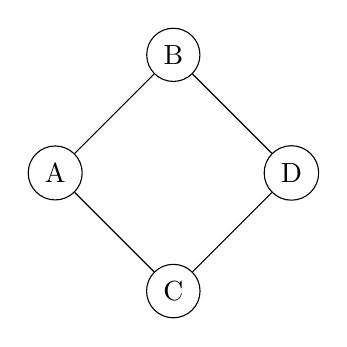
\begin{tikzpicture}[scale=1.5]
            % Define vertices
            \node[circle, draw] (A) at (0, 0) {A};
            \node[circle, draw] (B) at (1, 1) {B};
            \node[circle, draw] (C) at (1, -1) {C};
            \node[circle, draw] (D) at (2, 0) {D};

            % Draw edges
            \draw (A) -- (B);
            \draw (A) -- (C);
            \draw (B) -- (D);
            \draw (C) -- (D);
        \end{tikzpicture}
        \caption{Graph representation of vertices A, B, C, and D.}
    \end{minipage}%
    \hfill
    % Create a minipage for the adjacency matrix
    \begin{minipage}{0.45\textwidth}
        \[
        A =
        \begin{bmatrix}
        0 & 1 & 1 & 0 \\
        1 & 0 & 0 & 1 \\
        1 & 0 & 0 & 1 \\
        0 & 1 & 1 & 0 \\
        \end{bmatrix}
        \]
        \caption{Adjacency matrix corresponding to the graph.}
    \end{minipage}
\end{figure}

By using these adjacency matrices and leveraging linear algebra techniques, we can calculate triangle counts more efficiently. 
One simple method using the adjacency matrix is to use the following formula:

\[
\Delta = \frac{1}{6} \mathrm{trace}(A^3)
\]

This formula is derived from the fact that the diagonal elements of \(A^3\) count the number of length-three paths (i.e. triangles) that each vertex participates in.
Thus, in taking the trace, we get the sum of all these triangles, which after scaling, yields the global triangle count.

To compute $A^3$, we first need to calculate $A^2$ (which takes $O(n^3)$ for an $n \times n$ matrix) and then multiply $A^2$ by $A$ (also $O(n^3)$).
Thus, the total complexity for computing $A^3$ is $O(n^3)$.
After computing $A^3$, calculating the trace takes $O(n)$, as we need to iterate over the $n$ diagonal elements.
Thus, the overall runtime complexity for the operation is $O(n^3)$.

\subsubsubsection{Strassen's Algorithm}

This runtime analysis assumes that matrix multiplication is performed using the standard algorithm.
However, more sophisticated techniques, such as Strassen's algorithm \cite{strassen_gaussian_1969}, can reduce matrix multiplication time.
In this algorithm, that is used on For large, square matrices, such as undirected sociomatrices, each matrix is divided into smaller submatrices on which a series additions and multiplications are performed.
This process requires only seven multiplications of these smaller matrices instead of the eight that are typical in standard matrix multiplication.
Thus, on large matrices, this leads to a significant speedup.

Specifically, Strassen's algorithm reduces the complexity of multiplying two $n \times n$ matrices to approximately $O(n^{\log_2 7})$, which is about $O(n^{2.81})$.
Computing $A^2$ using Strassen's algorithm will take $O(n^{\log_2 7})$.
Then, multiplying $A^2$ by $A$ again takes $O(n^{2.81})$.
Therefore, the total complexity for computing $A^3$ with Strassen's algorithm is $O(n^{\log_2 7}) + O(n^{\log_2 7}) = O(n^{\log_2 7})$, or roughly $O(n^{2.81})$.

\subsubsubsection{EigenTriangle Algorithm}

Another significant approach in triangle counting is the use of spectral methods.
One such method is the EigenTriangle algorithm \cite{tsourakakis_fast_2008}, which estimates the triangle count $\Delta$ by considering the spectral decomposition of the adjacency matrix $A$.

The EigenTriangle algorithm is based on the observation that the number of triangles in a graph is closely related to the spectrum of its adjacency matrix.
In particular, the adjacency matrix $A$ is decomposed as:

\[
A = U \Lambda U^T
\]

where $U$ is a matrix whose columns are the eigenvectors of $A$, and $\Lambda$ is a diagonal matrix containing the corresponding eigenvalues.

Once the decomposition is performed, the number of triangles can be computed exactly using $\Delta = \frac{1}{6} \sum_{i=1}^{n} \lambda_i^3$, and can be estimated using:

\[
\Delta \approx \frac{1}{6} \sum_{i=1}^{k} \lambda_i^3
\]

where $\lambda_i$ are the $k$ top eigenvalues of the adjacency matrix.
The runtime of EigenTriangle is dominated by the cost of computing the top $k$ eigenvalues and eigenvectors of $A$, which can be done in $O(k m)$, where $m$ is the number of edges and $k$ is typically much smaller than the number of nodes $n$.
This is a substantial improvement over the complexity of direct methods like $\mathrm{trace}(A^3)$.

\subsubsubsection{TraceTriangle Algorithm}

The TraceTriangle algorithm \cite{avron_counting_2010} is a randomized algorithm designed for efficient triangle estimation in large graphs.
It leverages trace-based techniques, which compute the trace of matrix powers to approximate the number of triangles.
Specifically, the algorithm relies on the previously mentioned property: $\Delta = \frac{1}{6} \mathrm{trace}(A^3)$ where $A$ is the adjacency matrix of the graph and $\Delta$ is the number of triangles.
However, rather than computing the full matrix multiplication $A^3$, which is computationally expensive for large graphs, the TraceTriangle algorithm uses a randomized approach to approximate this trace, significantly reducing computation time.

Comparing TraceTriangle to the EigenTriangle algorithm, TraceTriangle achieves higher accuracy across multiple types of graphs.
Despite this accuracy advantage, EigenTriangle tends to run more quickly than TraceTriangle on large graphs.
That said, one significant advantage of TraceTriangle is its potential for parallelization, which EigenTriangle lacks.
This allows TraceTriangle to scale more effectively with the size of the graph, ultimately reducing the speed advantage of EigenTriangle in larger computations.

\subsubsection{Sampling Methods}

One of the most effective ways to estimate triangle counts in large, sparse graphs is through sampling methods.
These methods rely on randomly selecting edges or vertices and then inspecting their local neighborhoods for the presence of triangles.
Sampling-based techniques are particularly useful in scenarios where calculating the exact triangle count is computationally expensive or unnecessary.

Additionally, sampling algorithms often provide tunable accuracy, allowing for a trade-off between precision and performance, making them ideal for processing large-scale networks.

\subsubsubsection{Edge Sampling}

In edge sampling, we randomly sample a subset of edges from the graph, count the number of triangles in the subgraph, and scale up to reach our estimate.

One key edge sampling algorithm is Doulion \cite{tsourakakis_doulion_2009}, in which each edge in $G$ is sampled with probability $p$.
As all triangles consist of three edges, meaning that all triangles in $G$ have probability $p^3$ of being counted.
Thus, the number of triangles counted is scaled by $\frac{1}{p^3}$ to achieve a final estimate.

\subsubsubsection{Wedge Sampling}

Wedge sampling \cite{seshadhri_triadic_2013} focuses on counting wedges—triplets of nodes that form two edges but not necessarily a triangle.
A wedge is defined by three vertices $(u, v, w)$ where $u$ is adjacent to both $v$ and $w$, but $v$ and $w$ may or may not be adjacent.
Once wedges are sampled, the algorithm checks how many of them are closed (i.e., form triangles).

The number of triangles can then be estimated by multiplying the number of closed wedges by the fraction of all wedges that were closed in the sample.
Wedge sampling tends to work well in graphs with a large number of high-degree vertices, where it becomes easier to sample many wedges at once, but unlike edge sampling, it cannot be efficiently done using data structures like adjacency matrices or adjacency lists.
Thus, wedge sampling comes with an additional preprocessing step that adds to runtime.

\subsection{General Algorithmic Strategies}

Beyond specific algorithms for triangle counting, various general techniques from theoretical computer science have been adapted for this problem, particularly in designing faster algorithms.

\subsubsection{Variance Reduction}

Variance reduction \cite{prescott_monte_1965} is another general technique that can be applied to triangle estimation, improving accuracy without increasing the number of samples needed.

Variance reduction methods aim to reduce the spread (or variance) of estimations, leading to more reliable results even with fewer samples.
This is particularly important in large-scale graphs, where taking a high number of samples may be computationally infeasible.

\subsubsubsection{Importance Sampling}

One example of a variance reduction method is importance sampling.
When estimating a metric relating to a large population using uniform sampling, where all edges/nodes/wedges/etc. are sampled with the same probability, often a very large number of samples is required to ensure a good relative approximation \cite{lovasz_large_2012}.
This is because uniform sampling does not prioritize areas of the graph that may have a disproportionately large impact on the estimate.
Consequently, the computational cost can be high for achieving a desired accuracy level in many cases.

When using importance sampling \cite{motwani_randomized_1995}, the process is improved by sampling higher-interest nodes with higher probability, focusing computational effort on the most ``important" parts of a graph.
The key idea behind importance sampling is to bias the sampling distribution towards more informative areas of the graph.
For instance, in a graph where certain nodes are highly connected or play a critical role in the overall structure, importance sampling would prioritize these nodes to reduce the variance of the estimates.

\subsubsection{Learning-Augmented Algorithms}

A learning-augmented algorithm \cite{roughgarden_algorithms_2020} is an algorithm that uses a prediction to boost its performance.
Whereas most algorithms take only the problem their input, learning-augmented algorithms also accept an extra piece of information—usually a prediction about some part of the solution.
The algorithm then uses this prediction to run faster or produce better results.

An example of a learning-augmented algorithm is its use in the maximum weight matching problem.
The maximum weight matching problem \cite{duan_linear-time_2014} is the problem of finding a matching in which the sum of weights is maximized in a weighted graph.
The typical solution for this problem, the Hungarian algorithm, runs in $O(m\sqrt{n})$ time.

When a learning-augmented approach \cite{dinitz_faster_2021} is applied however, where machine-learned predictions are used to ``warm-start" the algorithm, that runtime is significantly reduced when the predictions are accurate.
When the predictions are inaccurate, the runtime is simply the same as in the Hungarian algorithm.

In general, this method can be highly effective, as accurate predictions can significantly enhance algorithms' efficiency or result quality.

\newpage
\bibliographystyle{plain}
\bibliography{thesis_bib}

\end{document}
